\section{Einführung in Gleichrichter und Grundsystematik}

Gleichrichter dienen der Umwandlung von Wechselspannung in Gleichspannung.
Sie bilden die Eingangsstufe nahezu aller leistungselektronischen Systeme,
insbesondere in Netzteilen, Umrichtern und elektrischen Antrieben.

Je nach Schaltungstopologie, Pulszahl und Steuerart ergeben sich sehr unterschiedliche
Eigenschaften hinsichtlich Mittelwert, Restwelligkeit, Netzrückwirkungen und Stellbarkeit.

\subsection{Systematik der Gleichrichterbezeichnungen}

Die Bezeichnungen der Gleichrichter folgen einer einheitlichen Nomenklatur,
die unmittelbar Auskunft über Aufbau und Funktion gibt:

\begin{itemize}
\item \textbf{M} = Mittelpunktschaltung,
\item \textbf{B} = Brückenschaltung,
\item \textbf{Zahl} = Pulszahl $p$ pro Netzperiode,
\item \textbf{U} = ungesteuert (Dioden),
\item \textbf{C} = gesteuert (Thyristoren).
\end{itemize}

Beispiele:
\begin{itemize}
\item M1U: Einpuls, Mittelpunkt, ungesteuert,
\item B2U: Zweipuls, Brücke, ungesteuert,
\item B6C: Sechspuls, Brücke, gesteuert.
\end{itemize}

Die Pulszahl bestimmt die Frequenz der Gleichspannungswelligkeit
und damit die Qualität der erzeugten Gleichspannung.

\crd{\textrightarrow\ M/B beschreibt die Topologie, die Zahl die Pulszahl, U/C die Steuerart.}

\subsection{Grundklassifikation der Gleichrichter}

Man unterscheidet grundsätzlich zwei Hauptklassen:

\begin{itemize}
\item \textbf{Ungesteuerte Gleichrichter (U)}:  
Dioden, keine Stellmöglichkeit der Ausgangsspannung.

\item \textbf{Gesteuerte Gleichrichter (C)}:  
Thyristoren, Stellgrösse ist der Zündwinkel $\alpha$.
\end{itemize}

Bei gesteuerten Gleichrichtern ist der Mittelwert der Gleichspannung
proportional zu $\cos\alpha$.
Für $\alpha > 90^\circ$ ist Rückspeisebetrieb möglich.

\subsection{Einfluss von Induktivität und Kapazität auf den Betrieb}

In realen Anwendungen werden Induktivität $L$ und Kapazität $C$ eingesetzt,
um das Verhalten des Gleichrichters gezielt zu beeinflussen.
Sie bestimmen wesentlich die Stromform, die Spannungswelligkeit
sowie die Netzrückwirkungen.

Man unterscheidet drei Grundfälle:

\begin{itemize}
\item \textbf{C-Glättung (kapazitive Last)},
\item \textbf{L-Glättung (induktive Last)},
\item \textbf{LC-Glättung (Filter)}.
\end{itemize}

Der gewählte Lasttyp bestimmt insbesondere:

\begin{itemize}
\item die Stromform $i_d(t)$ im Gleichrichter,
\item die Restwelligkeit der Gleichspannung $\Delta u_d$,
\item die Netzstromharmonischen,
\item den Leistungsfaktor $\lambda$,
\item die thermische Belastung der Halbleiter.
\end{itemize}

\subsubsection*{C-Glättung (kapazitive Last)}

Der Kondensator lädt sich in jeder Leitphase auf den momentanen Scheitelwert
der Gleichspannung auf und entlädt sich zwischen den Leitphasen über die Last.

Näherung für den Spannungsrippel:
\[
\cbl{\Delta u_d \approx \frac{I_d}{f_r \, C}}
\]
mit:
\begin{itemize}
\item $I_d$: mittlerer Gleichstrom,
\item $f_r = p f$: Ripple-Frequenz der Gleichspannung,
\item $p$: Pulszahl des Gleichrichters,
\item $f$: Netzfrequenz,
\item $C$: Kapazität des Kondensators.
\end{itemize}

Mittelwert der Gleichspannung:
\[
\cbl{u_d \approx \hat U_d - \frac{\Delta u_d}{2}}
\]
mit:
\begin{itemize}
\item $\hat U_d$: Scheitelwert der gleichgerichteten Spannung.
\end{itemize}

Typische Konsequenzen:
\begin{itemize}
\item Sehr kurze Leitwinkel $\Rightarrow$ hohe Spitzenströme:
\[
\cbl{i_{D,\max} \gg I_d}
\]
\item Starke Verzerrung des Netzstroms.
\item Schlechter Leistungsfaktor:
\[
\cbl{\lambda = \frac{P}{U_{\mathrm{RMS}} I_{\mathrm{RMS}}} \ll 1}
\]
\end{itemize}

\subsubsection*{L-Glättung (induktive Last)}

Die Induktivität erzwingt eine nahezu konstante Stromform.
Im stationären Betrieb gilt für die mittlere Induktorspannung:

\[
\cbl{\overline{u_L} = \frac{1}{T}\int_0^T u_L(t)\, dt = 0}
\]

Mit:
\[
u_L(t) = L \frac{di_d(t)}{dt}
\]

Daraus folgt für den Mittelwert der Gleichspannung:
\[
\cbl{u_d = \overline{u_{\mathrm{gr}}(t)}}
\]
mit:
\begin{itemize}
\item $u_{\mathrm{gr}}(t)$: momentane gleichgerichtete Spannung.
\end{itemize}

Stromwelligkeit:
\[
\cbl{\Delta i_d \approx \frac{\Delta u_d}{\omega L}}
\]

Typische Konsequenzen:
\begin{itemize}
\item Nahezu konstanter Gleichstrom:
\[
\cbl{i_d(t) \approx I_d = \text{konstant}}
\]
\item Rechteckförmige Netzströme bei Mehrpuls-Gleichrichtern.
\item Geringere Oberschwingungen als bei C-Glättung.
\item Besserer Leistungsfaktor:
\[
\cbl{\lambda \uparrow}
\]
\end{itemize}

\subsubsection*{LC-Glättung (Tiefpassfilter)}

Die Kombination aus Serieninduktivität und Parallel-Kondensator
bildet ein Tiefpassfilter für die Gleichspannung.

Grenzfrequenz des Filters:
\[
\cbl{\omega_0 = \frac{1}{\sqrt{LC}}}
\qquad
f_0 = \frac{1}{2\pi\sqrt{LC}}
\]

Übertragungsverhalten:
\[
|H(j\omega)| \approx
\begin{cases}
1, & \omega \ll \omega_0, \\
\downarrow, & \omega \gg \omega_0.
\end{cases}
\]

Dämpfung der Ripple-Komponente:
\[
\cbl{\Delta u_d \propto |H(j\omega_r)|}
\]
mit:
\begin{itemize}
\item $\omega_r = 2\pi f_r$: Ripple-Kreisfrequenz.
\end{itemize}

Typische Konsequenzen:
\begin{itemize}
\item Sehr geringe Restwelligkeit der Gleichspannung.
\item Gute Strom- und Spannungsqualität.
\item Höherer Bauteilaufwand.
\end{itemize}


\subsection{Ziel der folgenden Kapitel}

In den folgenden Kapiteln werden systematisch behandelt:

\begin{itemize}
\item Einpuls-Gleichrichter (M1U, M1C),
\item Zweipuls-Gleichrichter (B2U, B2C),
\item Dreiphasige Gleichrichter (B6U, B6C),
\item Einfluss von Last, Steuerung und Netzinduktivität,
\item Netzrückwirkungen und Harmonische.
\end{itemize}

Ziel ist eine einheitliche Beschreibung aller Gleichrichter
auf Basis von:

\begin{itemize}
\item Pulszahl $p$,
\item Steuerart (U/C),
\item Leitwinkel $\alpha$, $\beta$,
\item Mittelwert- und Verlustgleichungen.
\end{itemize}


\subsection{M1U: Ungesteuerter Einpuls-Gleichrichter}

% --- bestehende Grafik: Schaltung ---
\begin{center}
    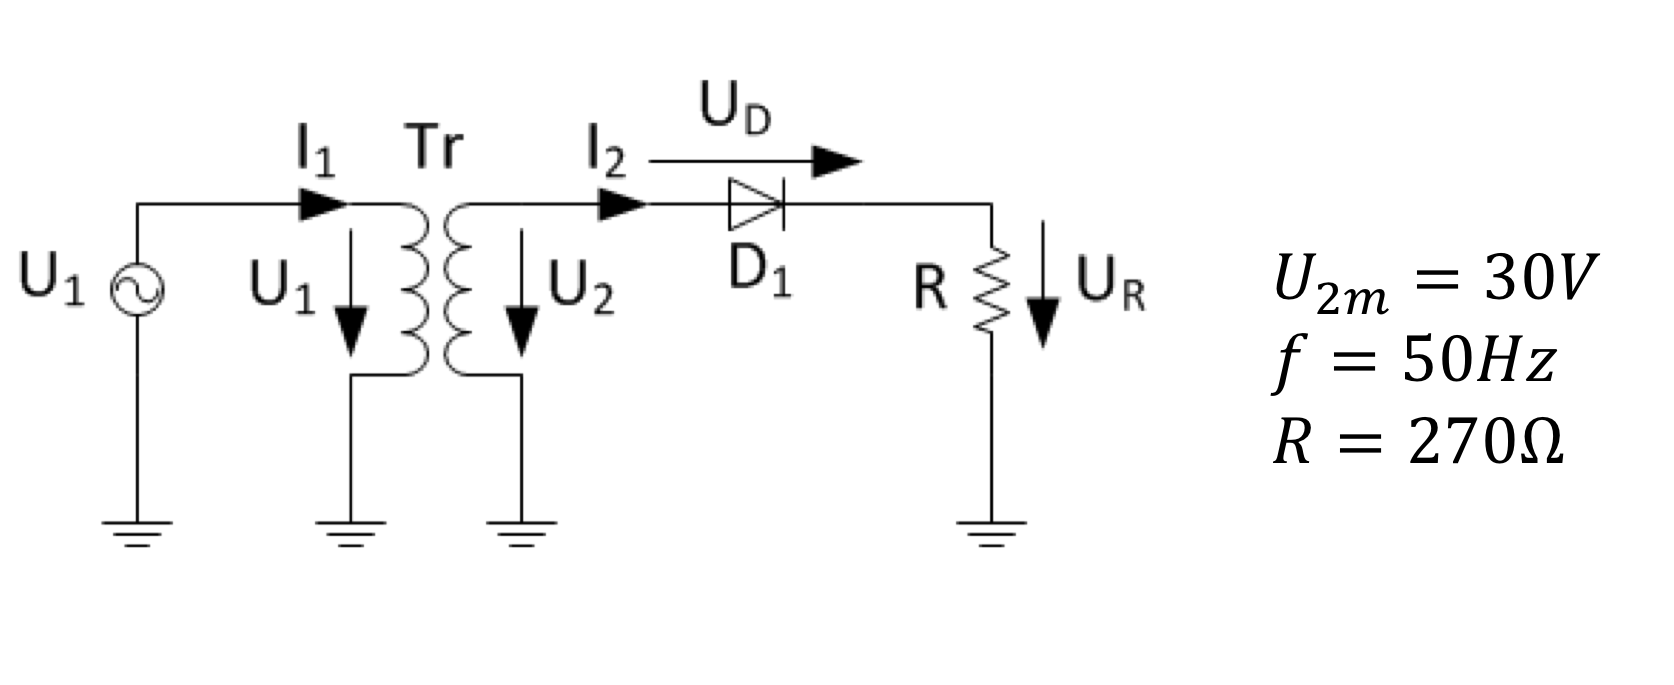
\includegraphics[width=0.85\linewidth]{images/M1U.png}
\end{center}

Der ungesteuerte Einpuls-Gleichrichter besteht aus einer Diode und einer einphasigen Wechselspannungsquelle.
Er arbeitet ohne Stellmöglichkeit und liefert eine pulsierende Gleichspannung mit der Pulszahl $p=1$.

Eingangsspannung:
\[
u_s(t) = \hat U \sin(\omega t)
\]
mit:
\begin{itemize}
\item $\hat U$: Scheitelwert der Eingangsspannung,
\item $\omega = 2\pi f$: Kreisfrequenz,
\item $f$: Netzfrequenz.
\end{itemize}

Momentane Ausgangsspannung:
\[
u_d(t) =
\begin{cases}
\hat U \sin(\omega t), & \sin(\omega t) \ge 0, \\
0, & \sin(\omega t) < 0.
\end{cases}
\]

Mittelwert der Gleichspannung:
\[
\cbl{\overline{u_d} = \frac{1}{2\pi}\int_0^{\pi} \hat U \sin\gamma \, d\gamma
= \frac{\hat U}{\pi}}
\]
mit:
\begin{itemize}
\item $\gamma = \omega t$: elektrischer Winkel.
\end{itemize}

Effektivwert der Ausgangsspannung:
\[
\cbl{U_{d,\mathrm{RMS}} = \sqrt{\frac{1}{2\pi}\int_0^{\pi} \hat U^2 \sin^2\gamma \, d\gamma}
= \frac{\hat U}{2}}
\]

Mittelwert des Gleichstroms bei ohmscher Last $R$:
\[
\cbl{I_d = \frac{\overline{u_d}}{R} = \frac{\hat U}{\pi R}}
\]

Effektivwert des Stroms:
\[
\cbl{I_{d,\mathrm{RMS}} = \frac{U_{d,\mathrm{RMS}}}{R} = \frac{\hat U}{2R}}
\]

Leistungsaufnahme an ohmscher Last:
\[
\cbl{P = R I_{d,\mathrm{RMS}}^2 = \frac{\hat U^2}{4R}}
\]

Eigenschaften:
\begin{itemize}
\item Keine Stellmöglichkeit der Ausgangsspannung.
\item Sehr hohe Restwelligkeit der Gleichspannung.
\item Geringe Gleichspannungsqualität.
\item Einfachste Gleichrichterschaltung.
\end{itemize}

% --- bestehende Grafik: Spannungsverlauf ---
\begin{center}
    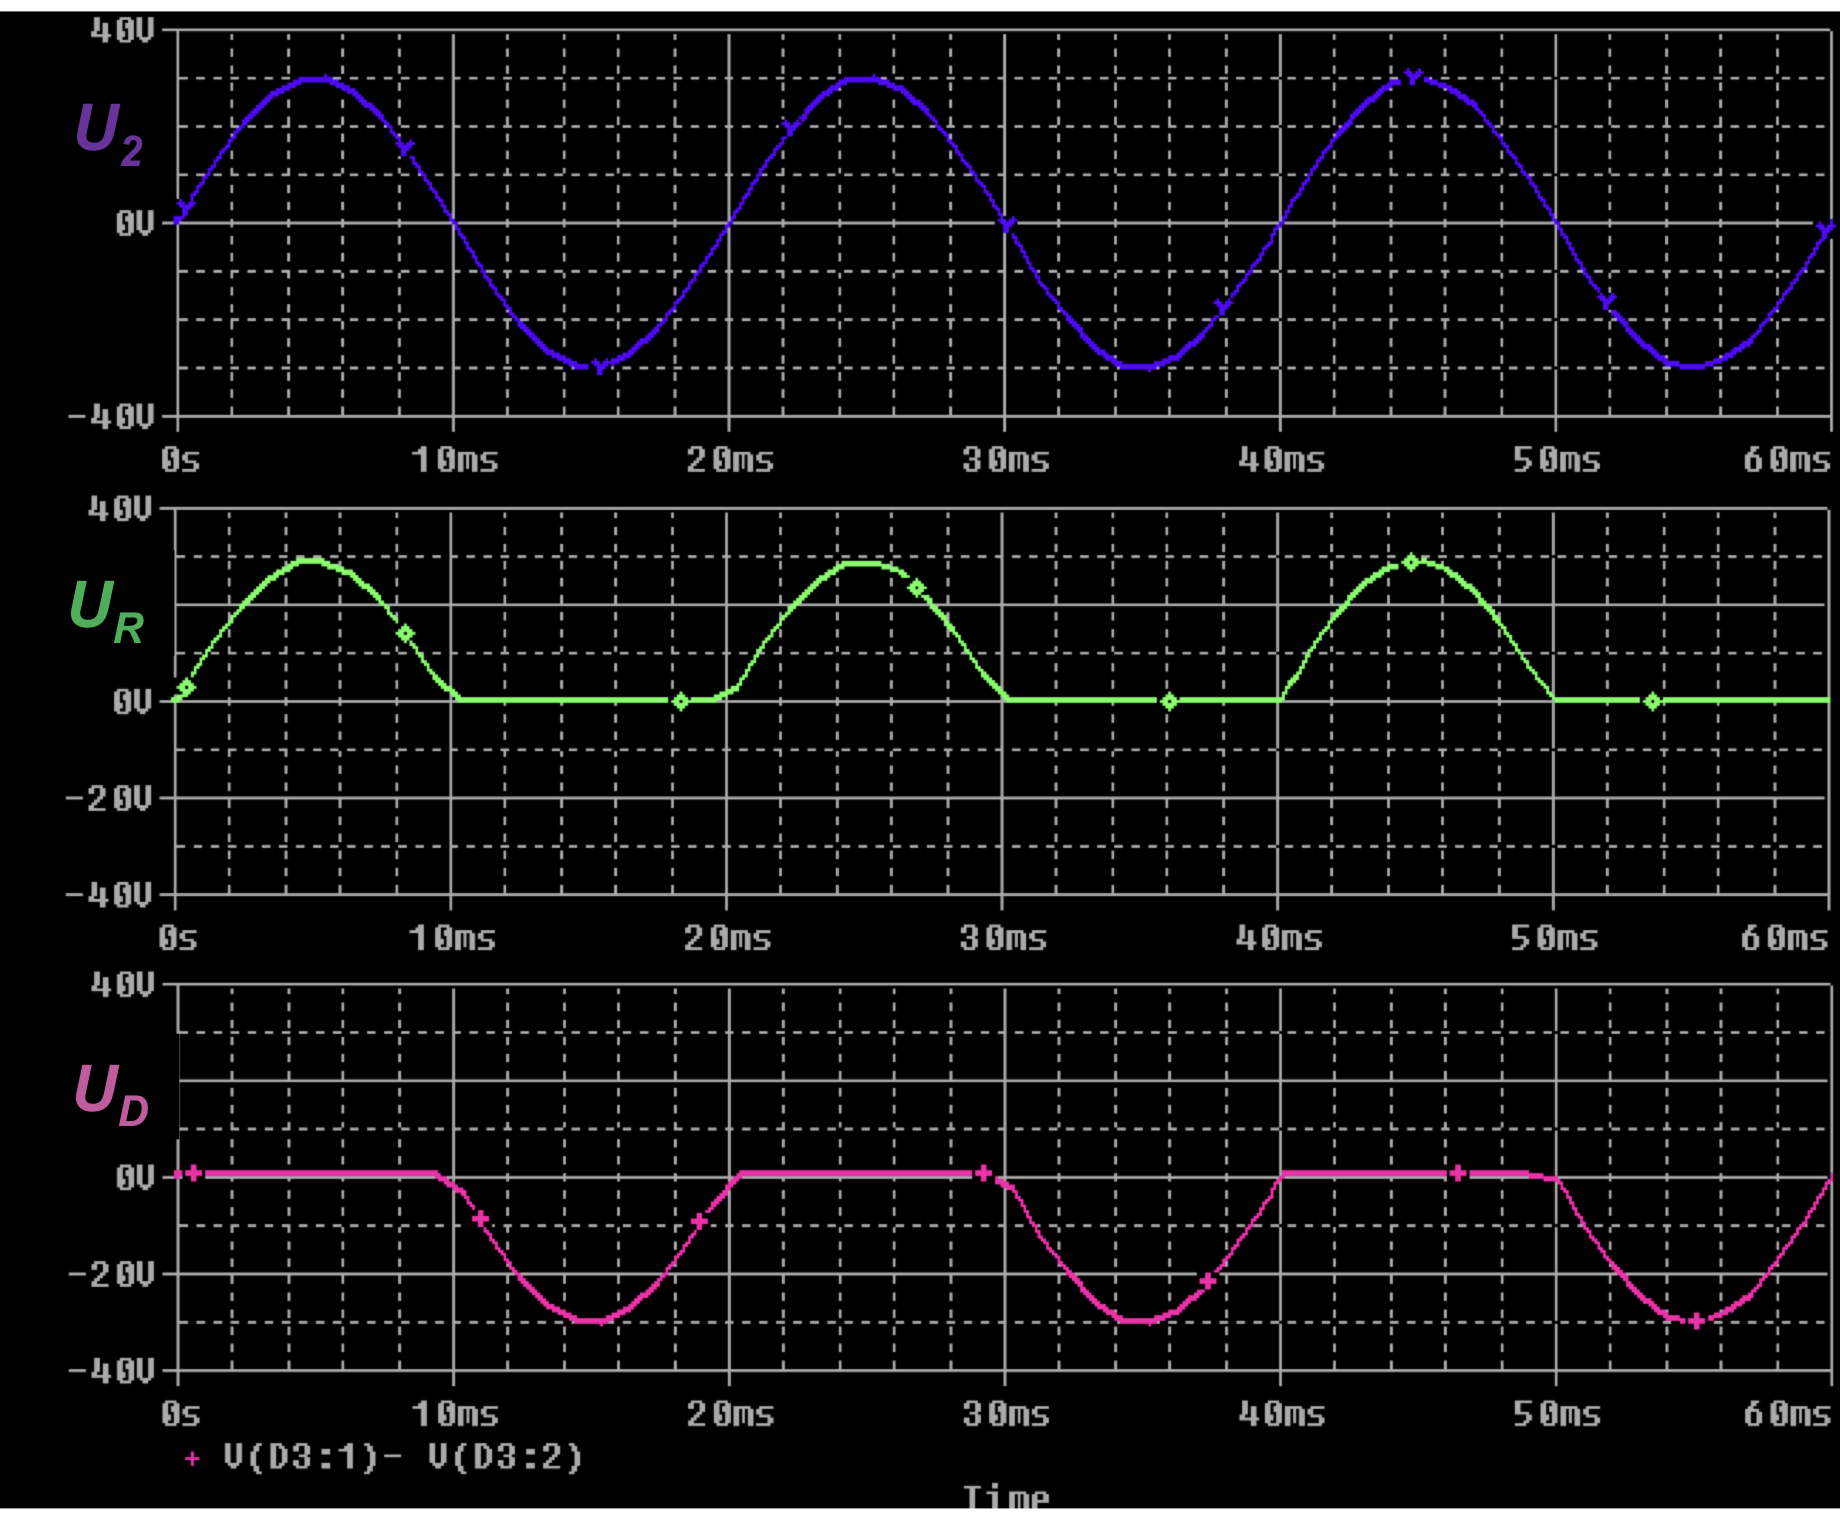
\includegraphics[width=0.85\linewidth]{images/M1U_verlauf.png}
\end{center}

\subsection{M1C: Gesteuerter Einpuls-Gleichrichter}

% --- bestehende Grafik: Schaltung ---
\begin{center}
    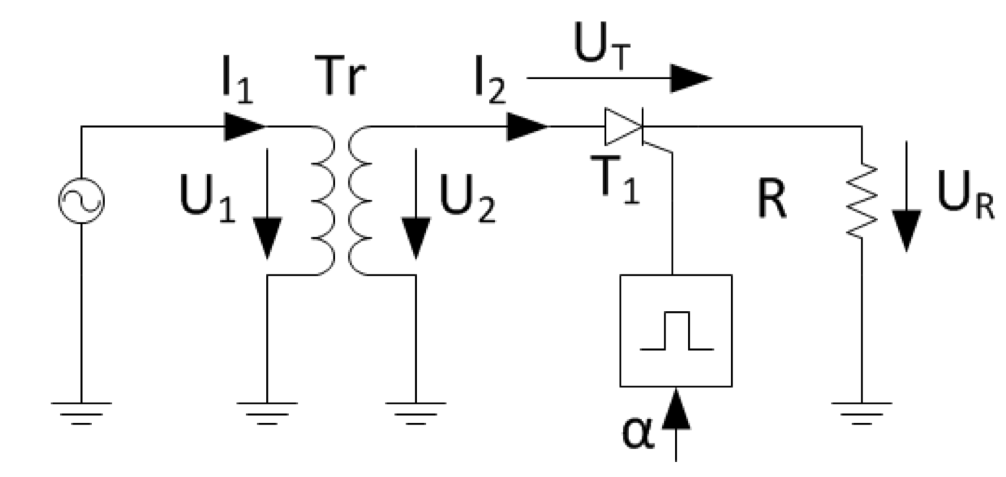
\includegraphics[width=0.85\linewidth]{images/M1C.png}
\end{center}

Der gesteuerte Einpuls-Gleichrichter ersetzt die Diode durch einen Thyristor.
Der Leitbeginn wird durch den Zündwinkel $\alpha$ gesteuert.

Eingangsspannung:
\[
u_s(t) = \hat U \sin(\omega t)
\]
mit:
\begin{itemize}
\item $\hat U$: Scheitelwert der Eingangsspannung,
\item $\omega = 2\pi f$: Kreisfrequenz,
\item $f$: Netzfrequenz.
\end{itemize}

Leitbedingung:
\[
\boxed{\omega t \ge \alpha}
\]

Momentane Ausgangsspannung:
\[
u_d(t) =
\begin{cases}
\hat U \sin(\omega t), & \omega t \ge \alpha, \\
0, & \omega t < \alpha.
\end{cases}
\]

Mittelwert der Gleichspannung:
\[
\cbl{\overline{u_d}
= \frac{1}{2\pi}\int_{\alpha}^{\pi} \hat U \sin\gamma \, d\gamma
= \frac{\hat U}{2\pi}(1+\cos\alpha)}
\]

Stellbereich:
\[
0 \le \alpha \le \pi
\]

Grenzfälle:
\[
\alpha = 0 \Rightarrow \overline{u_d} = \frac{\hat U}{\pi}
\]
\[
\alpha = \pi \Rightarrow \overline{u_d} = 0
\]

Mittelwert des Stroms bei ohmscher Last $R$:
\[
\cbl{I_d = \frac{\overline{u_d}}{R}
= \frac{\hat U}{2\pi R}(1+\cos\alpha)}
\]

Effektivwert der Ausgangsspannung:
\[
\cbl{U_{d,\mathrm{RMS}}
= \sqrt{\frac{1}{2\pi}\int_{\alpha}^{\pi} \hat U^2 \sin^2\gamma \, d\gamma}}
\]

Leistungsaufnahme an ohmscher Last:
\[
\cbl{P = R I_{d,\mathrm{RMS}}^2}
\]

Eigenschaften:
\begin{itemize}
\item Stellbare Gleichspannung über den Zündwinkel $\alpha$.
\item Bei $\alpha = 0$: Verhalten wie M1U.
\item Bei $\alpha > 90^\circ$: negativer Mittelwert möglich (in geeigneter Schaltung Rückspeisung).
\item Einfachster gesteuerter Gleichrichter.
\end{itemize}

% --- bestehende Grafik: Spannungsverlauf ---
\begin{center}
    \includegraphics[width=0.85\linewidth]{images/M1C_verlauf.png}
\end{center}

\subsection{B2U: Ungesteuerter Zweipuls-Gleichrichter}

% --- bestehende Grafik: Schaltung ---
\begin{center}
    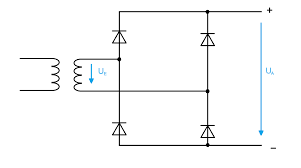
\includegraphics[width=0.85\linewidth]{images/B2U.png}
\end{center}

Der ungesteuerte Zweipuls-Gleichrichter ist eine vollwellige Brückenschaltung mit vier Dioden.
Er nutzt beide Halbwellen der Eingangsspannung und besitzt die Pulszahl $p=2$.

Eingangsspannung:
\[
u_s(t) = \hat U \sin(\omega t)
\]
mit:
\begin{itemize}
\item $\hat U$: Scheitelwert der Eingangsspannung,
\item $\omega = 2\pi f$: Kreisfrequenz,
\item $f$: Netzfrequenz.
\end{itemize}

Momentane Ausgangsspannung:
\[
u_d(t) = |u_s(t)| = |\hat U \sin(\omega t)|
\]

Mittelwert der Gleichspannung:
\[
\cbl{\overline{u_d}
= \frac{1}{\pi}\int_{0}^{\pi} \hat U \sin\gamma \, d\gamma
= \frac{2\hat U}{\pi}}
\]
mit:
\begin{itemize}
\item $\gamma = \omega t$: elektrischer Winkel.
\end{itemize}

Effektivwert der Ausgangsspannung:
\[
\cbl{U_{d,\mathrm{RMS}}
= \sqrt{\frac{1}{\pi}\int_{0}^{\pi} \hat U^2 \sin^2\gamma \, d\gamma}
= \frac{\hat U}{\sqrt{2}}}
\]

Mittelwert des Gleichstroms bei ohmscher Last $R$:
\[
\cbl{I_d = \frac{\overline{u_d}}{R} = \frac{2\hat U}{\pi R}}
\]

Effektivwert des Stroms:
\[
\cbl{I_{d,\mathrm{RMS}} = \frac{U_{d,\mathrm{RMS}}}{R}
= \frac{\hat U}{\sqrt{2}R}}
\]

Leistungsaufnahme an ohmscher Last:
\[
\cbl{P = R I_{d,\mathrm{RMS}}^2 = \frac{\hat U^2}{2R}}
\]

Restwelligkeit (Ripple-Faktor):
\[
\cbl{r = \frac{\sqrt{U_{d,\mathrm{RMS}}^2 - \overline{u_d}^2}}{\overline{u_d}}}
\]

Eigenschaften:
\begin{itemize}
\item Keine Stellmöglichkeit der Ausgangsspannung.
\item Deutlich geringere Welligkeit als beim M1U.
\item Doppelte Pulsfrequenz der Gleichspannung ($2f$).
\item Standard-Gleichrichter für einfache Anwendungen.
\end{itemize}

% --- bestehende Grafik: Spannungsverlauf ---
\begin{center}
    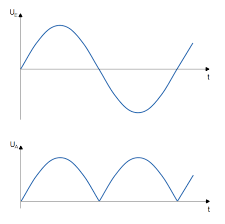
\includegraphics[width=0.85\linewidth]{images/B2U_verlauf.png}
\end{center}
\subsection{B2C: Gesteuerter Zweipuls-Gleichrichter}

% --- bestehende Grafik: Schaltung ---
\begin{center}
    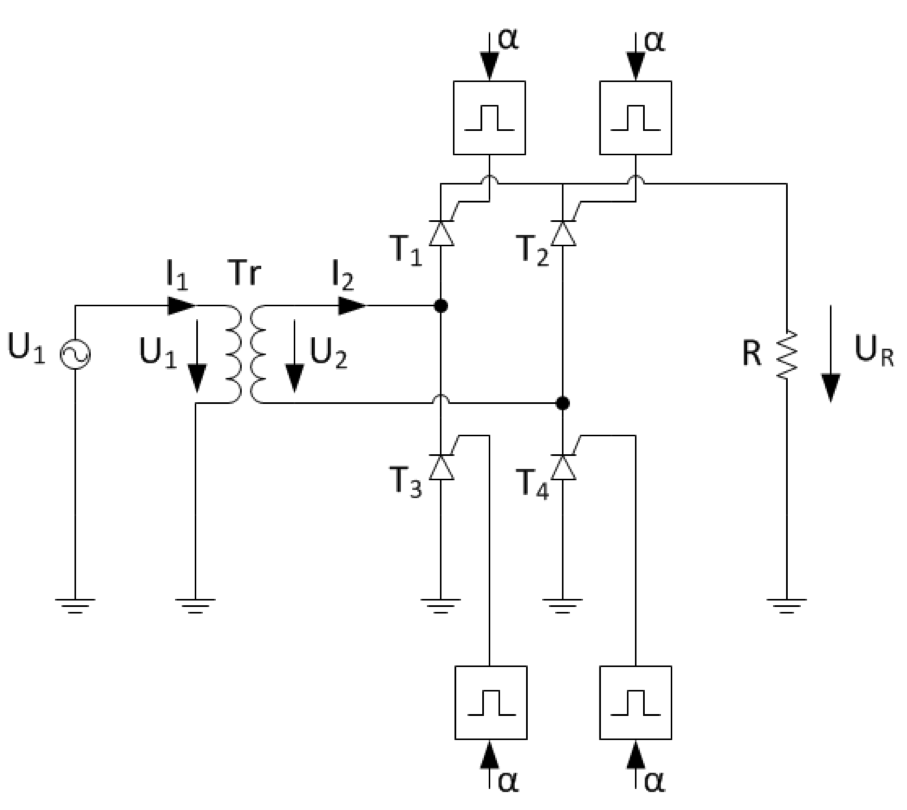
\includegraphics[width=0.85\linewidth]{images/B1C.png}
\end{center}

Der gesteuerte Zweipuls-Gleichrichter ersetzt die Dioden durch Thyristoren.
Der Leitbeginn wird über den Zündwinkel $\alpha$ gesteuert.

Eingangsspannung:
\[
u_s(t) = \hat U \sin(\omega t)
\]
mit:
\begin{itemize}
\item $\hat U$: Scheitelwert der Eingangsspannung,
\item $\omega = 2\pi f$: Kreisfrequenz,
\item $f$: Netzfrequenz.
\end{itemize}

Leitbedingung:
\[
\boxed{\omega t \ge \alpha}
\]

Momentane Ausgangsspannung:
\[
u_d(t) =
\begin{cases}
\hat U \sin(\omega t), & \omega t \ge \alpha, \\
0, & \omega t < \alpha.
\end{cases}
\]

Mittelwert der Gleichspannung:
\[
\cbl{\overline{u_d}
= \frac{1}{\pi}\int_{\alpha}^{\pi} \hat U \sin\gamma \, d\gamma
= \frac{2\hat U}{\pi}\cos\alpha}
\]

Stellbereich:
\[
0 \le \alpha \le \pi
\]

Grenzfälle:
\[
\alpha = 0 \Rightarrow \overline{u_d} = \frac{2\hat U}{\pi}
\]
\[
\alpha = \frac{\pi}{2} \Rightarrow \overline{u_d} = 0
\]
\[
\alpha > \frac{\pi}{2} \Rightarrow \overline{u_d} < 0 \quad \text{(Rückspeisebetrieb möglich)}
\]

Mittelwert des Stroms bei ohmscher Last $R$:
\[
\cbl{I_d = \frac{\overline{u_d}}{R}
= \frac{2\hat U}{\pi R}\cos\alpha}
\]

Effektivwert der Ausgangsspannung:
\[
\cbl{U_{d,\mathrm{RMS}}
= \sqrt{\frac{1}{\pi}\int_{\alpha}^{\pi} \hat U^2 \sin^2\gamma \, d\gamma}}
\]

Leistungsaufnahme an ohmscher Last:
\[
\cbl{P = R I_{d,\mathrm{RMS}}^2}
\]

Leistungsfaktor bei ohmscher Last:
\[
\cbl{\lambda = \frac{P}{U_{\mathrm{RMS}} I_{\mathrm{RMS}}}}
\]

Eigenschaften:
\begin{itemize}
\item Stellbare Gleichspannung über den Zündwinkel $\alpha$.
\item Mittelwert proportional zu $\cos\alpha$.
\item Rückspeisebetrieb für $\alpha > 90^\circ$.
\item Phasenanschnittsteuerung.
\end{itemize}

% --- bestehende Grafik: Zündwinkeldiagramm ---
\begin{center}
    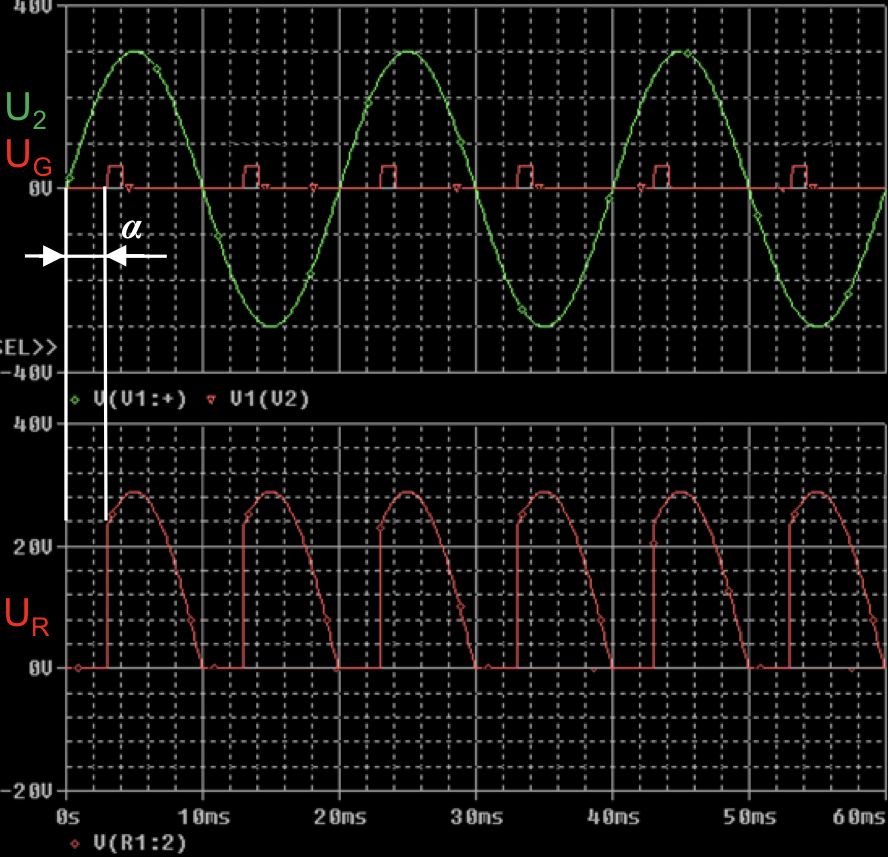
\includegraphics[width=0.85\linewidth]{images/B1C_Verlauf.png}
\end{center}

\subsection{B6U: Ungesteuerter Dreiphasen-Brückengleichrichter}

% --- bestehende Grafik: Schaltung ---
\begin{center}
    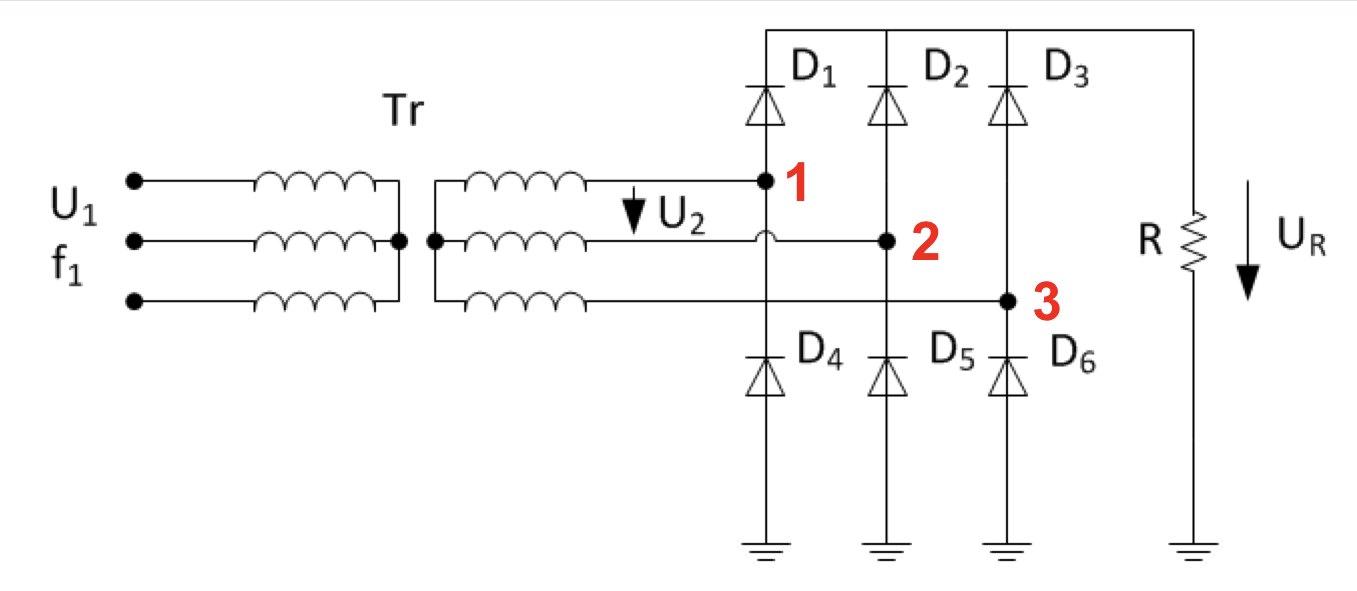
\includegraphics[width=0.65\linewidth]{images/B6U.png}
\end{center}

Der ungesteuerte Dreiphasen-Brückengleichrichter besteht aus sechs Dioden
und nutzt jeweils die beiden momentanen Leiterspannungen mit größtem Betrag.
Die Pulszahl beträgt $p=6$.

Eingangsspannungen:
\[
u_{ab}(t),\; u_{bc}(t),\; u_{ca}(t)
\]
mit:
\begin{itemize}
\item $U_{LL}$: Effektivwert der Leiterspannung,
\item $\hat U_{LL} = \sqrt{2} U_{LL}$: Scheitelwert der Leiterspannung,
\item $\omega = 2\pi f$: Kreisfrequenz,
\item $f$: Netzfrequenz.
\end{itemize}

Momentane Ausgangsspannung:
\[
u_d(t) = \max \{ u_{ab}(t),\, u_{bc}(t),\, u_{ca}(t),\, 0 \}
\]

Mittelwert der Gleichspannung:
\[
\cbl{\overline{u_d}
= \frac{3\sqrt{2}}{\pi} U_{LL}}
\]

Effektivwert der Gleichspannung (ideal, ohne Überlappung):
\[
\cbl{U_{d,\mathrm{RMS}}
= \sqrt{\frac{1}{2\pi}\int_0^{2\pi} u_d^2(\gamma)\, d\gamma}}
\]

Mittelwert des Gleichstroms bei ohmscher Last $R$:
\[
\cbl{I_d = \frac{\overline{u_d}}{R}
= \frac{3\sqrt{2}}{\pi}\frac{U_{LL}}{R}}
\]

Effektivwert des Gleichstroms:
\[
\cbl{I_{d,\mathrm{RMS}} = \frac{U_{d,\mathrm{RMS}}}{R}}
\]

Leistungsaufnahme an ohmscher Last:
\[
\cbl{P = R I_{d,\mathrm{RMS}}^2}
\]

Ripple-Frequenz der Gleichspannung:
\[
\cbl{f_r = p f = 6 f}
\]

Ripple-Faktor:
\[
\cbl{r = \frac{\sqrt{U_{d,\mathrm{RMS}}^2 - \overline{u_d}^2}}{\overline{u_d}}}
\]

Eigenschaften:
\begin{itemize}
\item Sehr geringe Restwelligkeit der Gleichspannung.
\item Hohe Gleichspannungsqualität.
\item Sehr gute Ausnutzung der Netzspannung.
\item Standard-Gleichrichter in Industrieanwendungen.
\end{itemize}

% --- bestehende Grafik: Spannungsverlauf ---
\begin{center}
    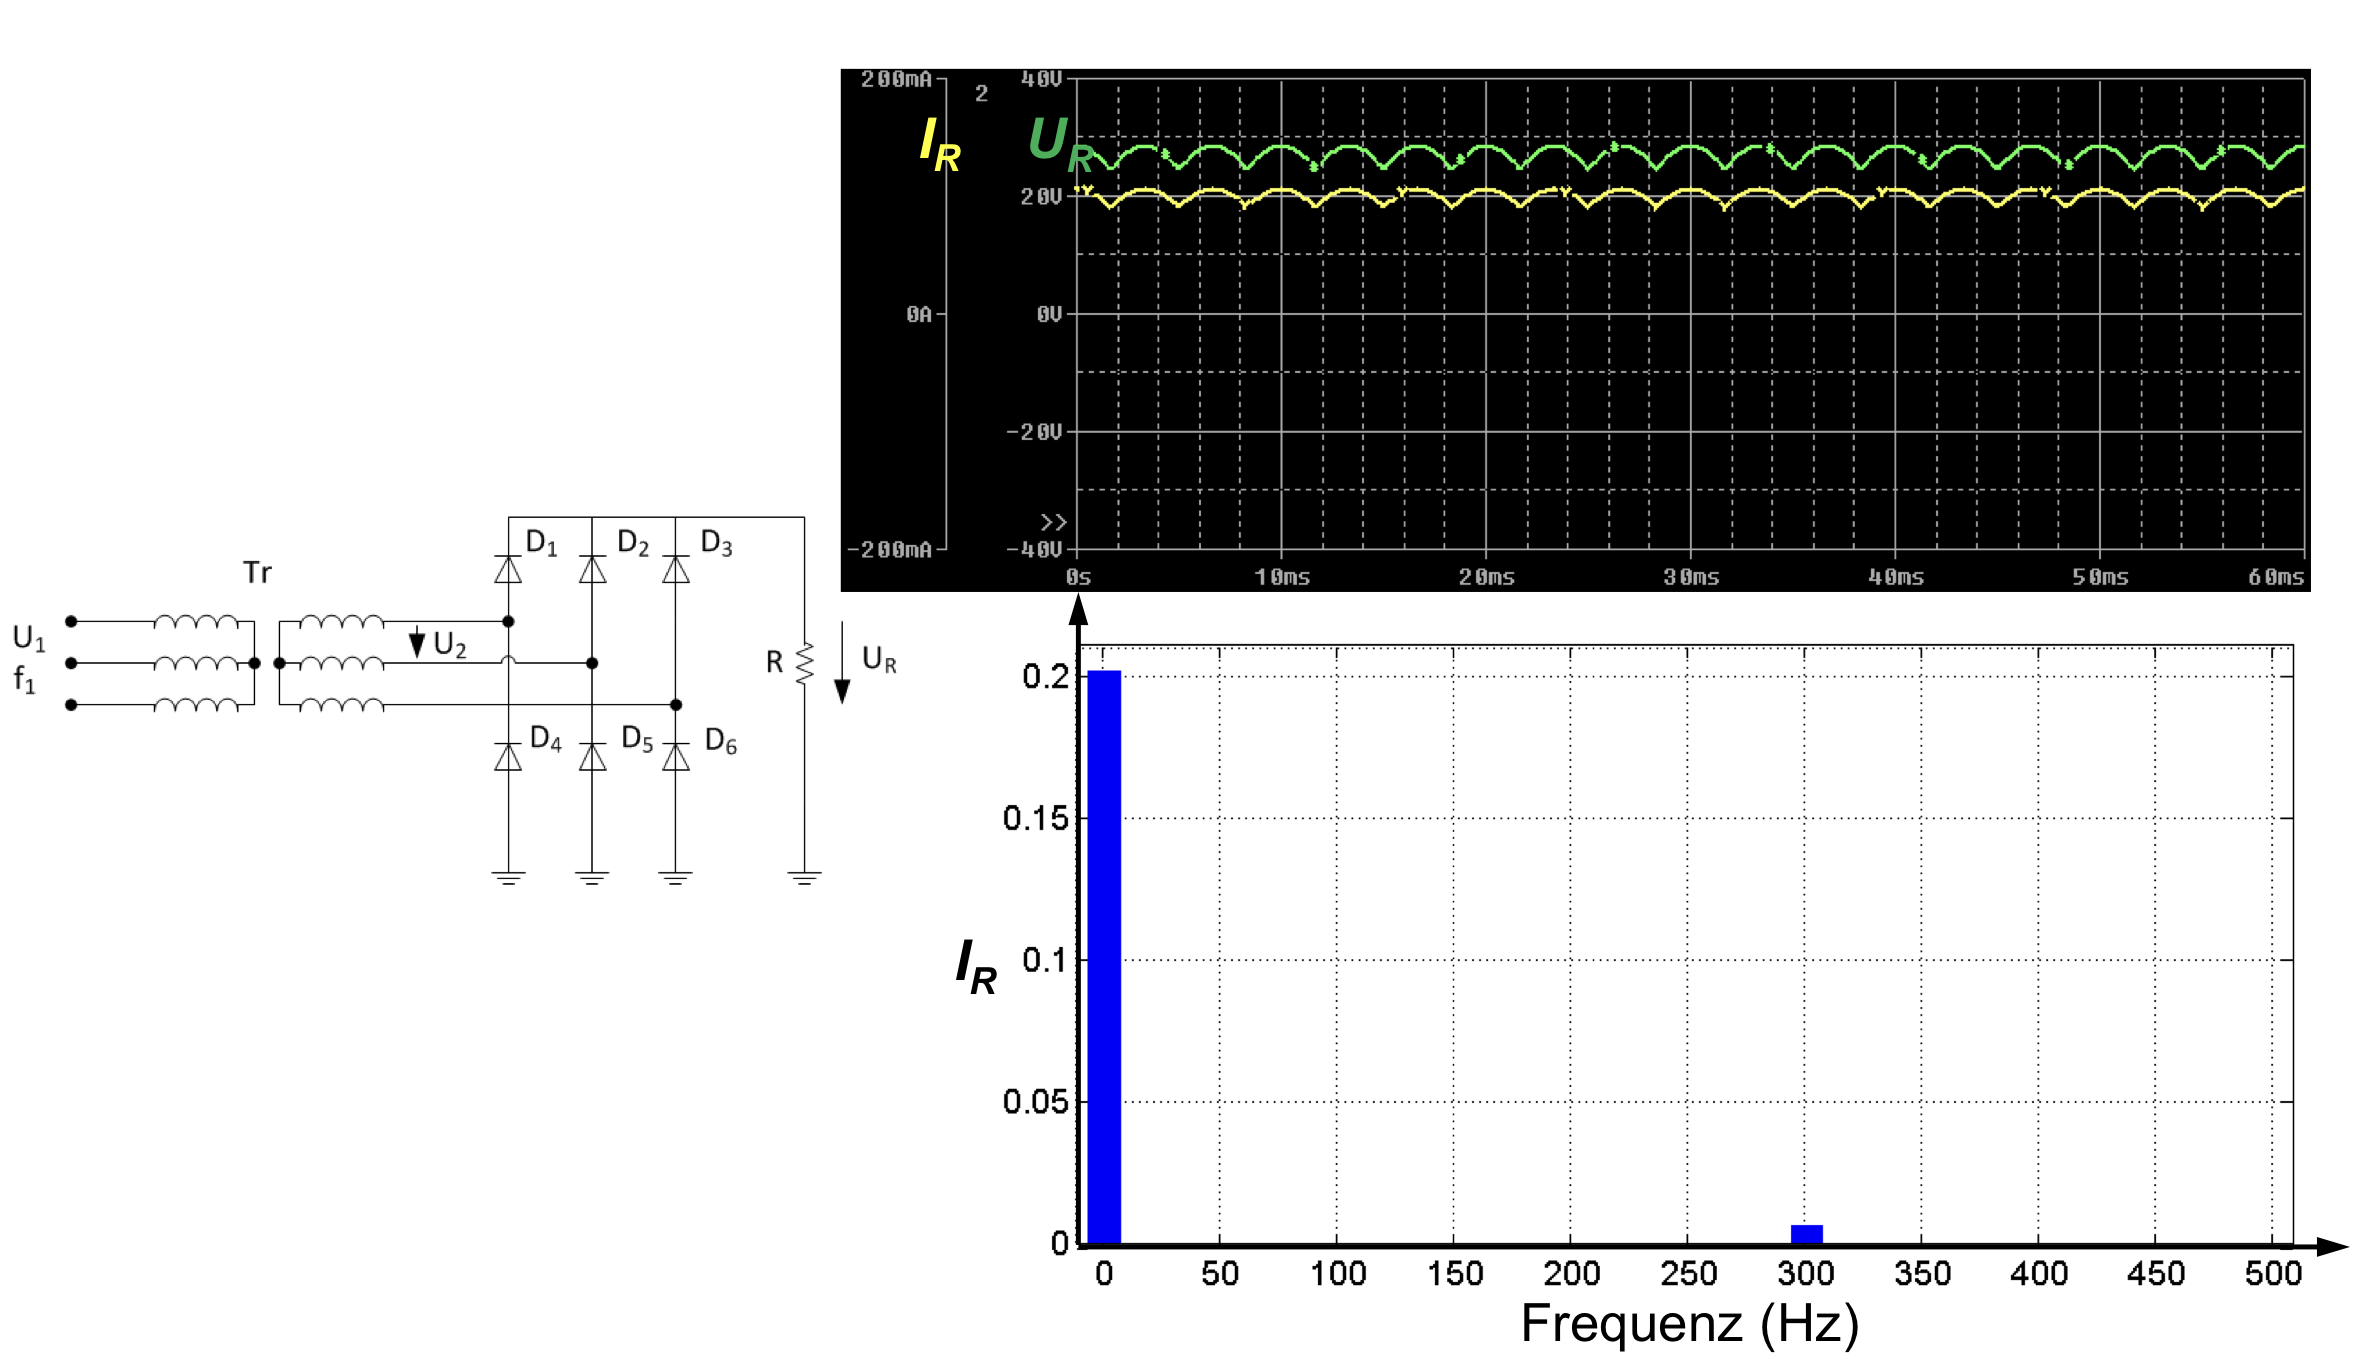
\includegraphics[width=0.85\linewidth]{images/B6U_verlauf.png}
\end{center}

\subsection{B6C: Gesteuerter Dreiphasen-Brückengleichrichter}

% --- bestehende Grafik: Schaltung ---
\begin{center}
    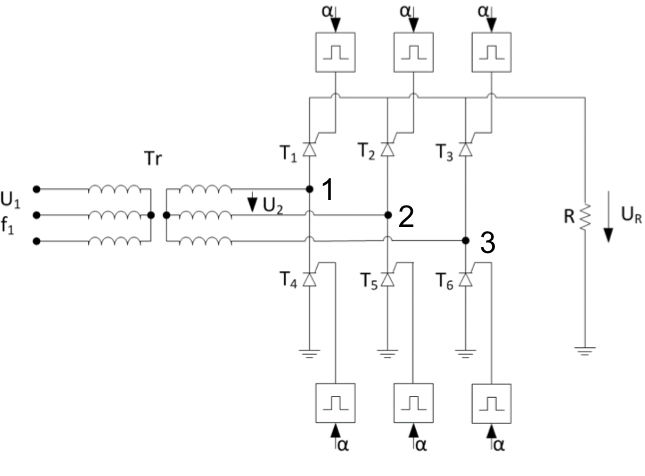
\includegraphics[width=0.65\linewidth]{images/B6C.png}
\end{center}

Der gesteuerte Dreiphasen-Brückengleichrichter ersetzt die Dioden durch Thyristoren.
Der Leitbeginn jedes Ventils wird über den Zündwinkel $\alpha$ gesteuert.

Eingangsspannungen:
\[
u_{ab}(t),\; u_{bc}(t),\; u_{ca}(t)
\]
mit:
\begin{itemize}
\item $U_{LL}$: Effektivwert der Leiterspannung,
\item $\hat U_{LL} = \sqrt{2} U_{LL}$: Scheitelwert der Leiterspannung,
\item $\omega = 2\pi f$: Kreisfrequenz,
\item $f$: Netzfrequenz.
\end{itemize}

Leitbedingung:
\[
\boxed{\omega t \ge \alpha}
\]

Momentane Ausgangsspannung:
\[
u_d(t) = u_{k\ell}(t)
\]
mit:
\begin{itemize}
\item $u_{k\ell}(t)$: jeweils aktive Leiterspannung des gerade leitenden Ventilpaares.
\end{itemize}

Mittelwert der Gleichspannung (ideal, ohne Überlappung):
\[
\cbl{\overline{u_d}
= \frac{3\sqrt{2}}{\pi} U_{LL} \cos\alpha}
\]

Stellbereich:
\[
0 \le \alpha \le \pi
\]

Grenzfälle:
\[
\alpha = 0 \Rightarrow \overline{u_d} = \frac{3\sqrt{2}}{\pi} U_{LL}
\]
\[
\alpha = \frac{\pi}{2} \Rightarrow \overline{u_d} = 0
\]
\[
\alpha > \frac{\pi}{2} \Rightarrow \overline{u_d} < 0 \quad \text{(Rückspeisebetrieb möglich)}
\]

Mittelwert des Gleichstroms bei ohmscher Last $R$:
\[
\cbl{I_d = \frac{\overline{u_d}}{R}
= \frac{3\sqrt{2}}{\pi}\frac{U_{LL}}{R}\cos\alpha}
\]

Effektivwert der Gleichspannung:
\[
\cbl{U_{d,\mathrm{RMS}}
= \sqrt{\frac{1}{2\pi}\int_0^{2\pi} u_d^2(\gamma)\, d\gamma}}
\]

Leistungsaufnahme an ohmscher Last:
\[
\cbl{P = R I_{d,\mathrm{RMS}}^2}
\]

Leistungsfaktor bei ohmscher Last:
\[
\cbl{\lambda = \frac{P}{\sqrt{3} U_{LL} I_{L,\mathrm{RMS}}}}
\]
mit:
\begin{itemize}
\item $I_{L,\mathrm{RMS}}$: Effektivwert des Leiterstroms.
\end{itemize}

Eigenschaften:
\begin{itemize}
\item Stellbare Gleichspannung über den Zündwinkel $\alpha$.
\item Mittelwert proportional zu $\cos\alpha$.
\item Rückspeisebetrieb für $\alpha > 90^\circ$.
\item Wichtigster gesteuerter Industrie-Gleichrichter.
\end{itemize}

% --- bestehende Grafik: Zeitverlauf ---
\begin{center}
    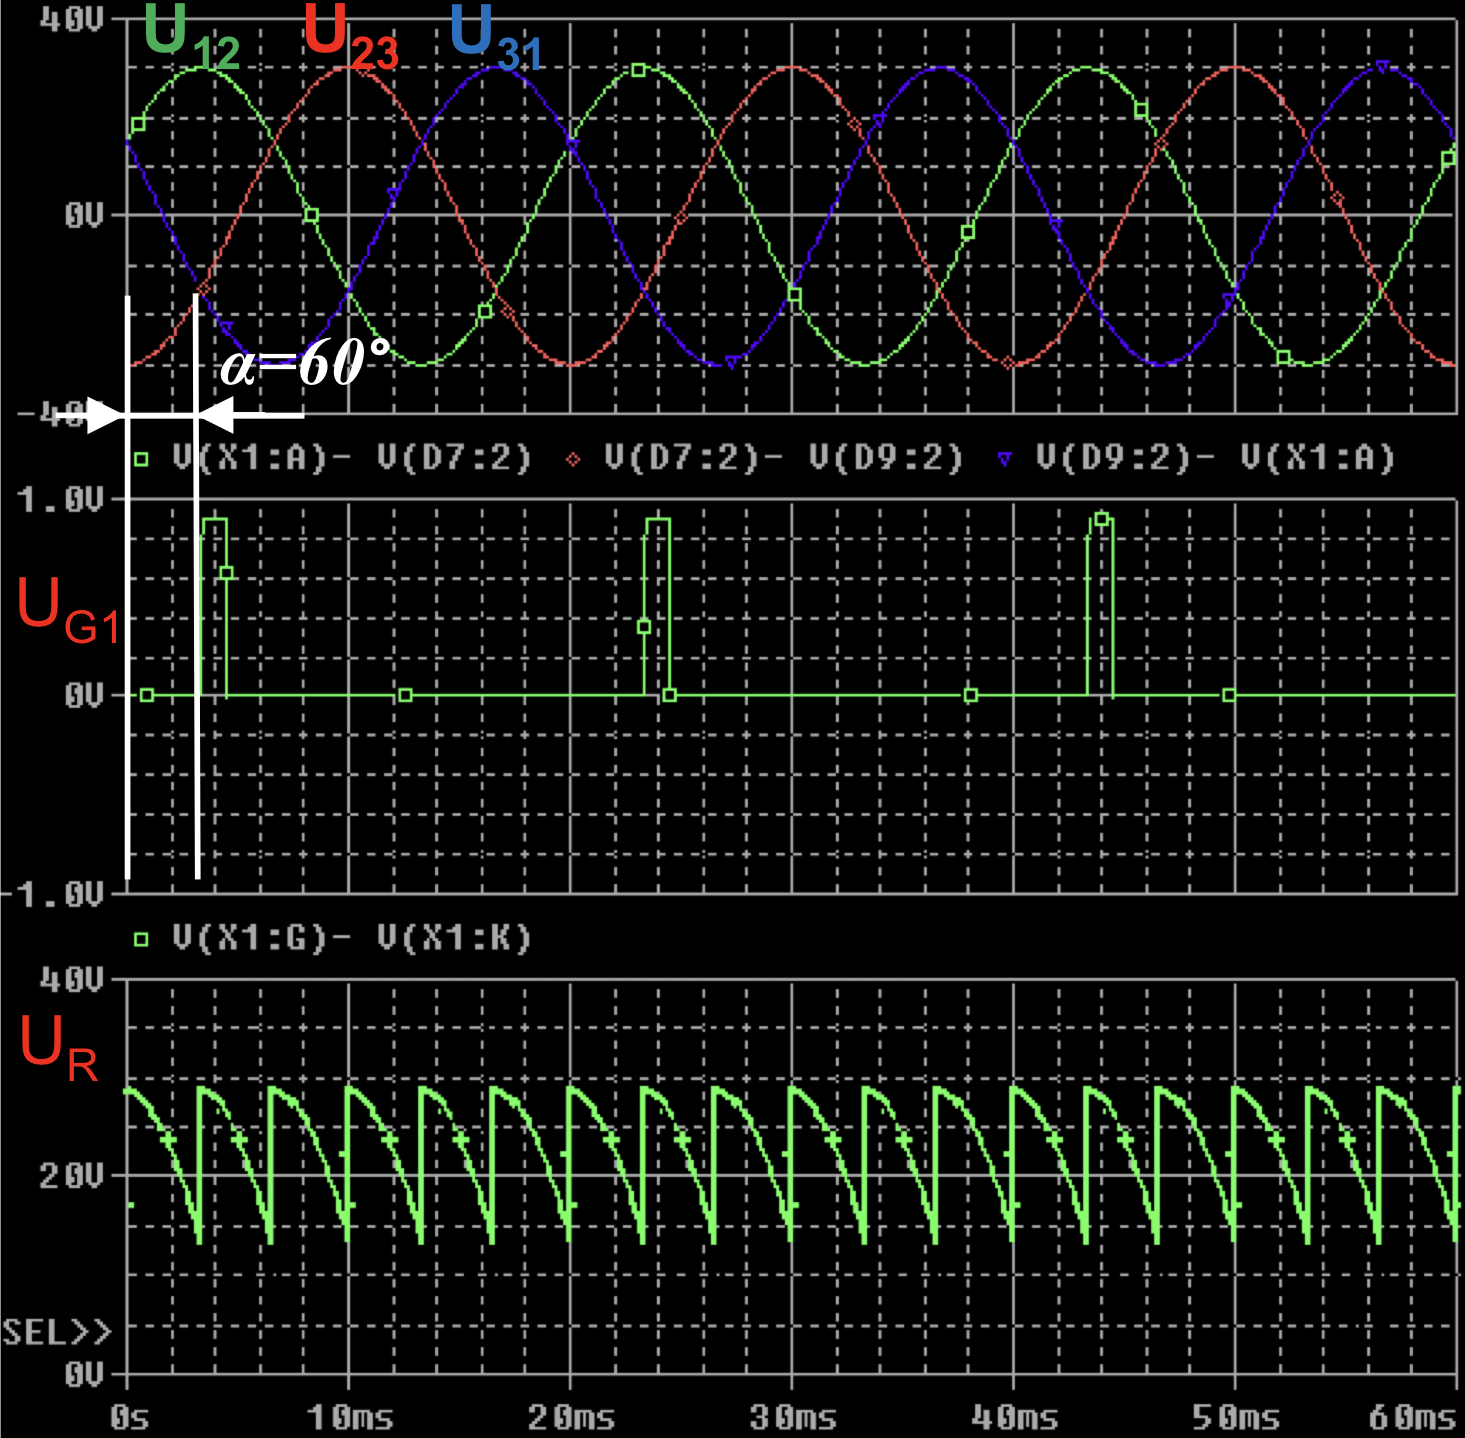
\includegraphics[width=0.85\linewidth]{images/B6C_Verlauf.png}
\end{center}
